\documentclass[final]{beamer}

\usepackage[scale=1.2]{beamerposter} % Use the beamerposter package for laying out the poster
\usepackage{caption} % Used to add caption to tabular
%\usepackage{lipsum} % Used for testing purposes
\usepackage{comment}
\usepackage{tcolorbox}
\usepackage[outline]{contour}
\usepackage{amsmath}
\captionsetup{labelformat=empty}

\definecolor{nibib1}{RGB}{50, 98, 150}
\definecolor{nibib2}{RGB}{57, 160, 237}
\definecolor{nibib3}{RGB}{100, 101, 105}
\definecolor{background}{RGB}{248, 248, 250}
\definecolor{umd}{RGB}{182, 19, 44}

\definecolor{decoder}{HTML}{97CAFF}
\definecolor{encoder}{HTML}{FFD28E}

\usetheme{confposter} % Use the confposter theme supplied with this template

\tcbset{
	colback=white,
    colframe=nibib3,
    coltext=black!80,
    coltitle=gray!5,
    fonttitle=\Large\bfseries,
    center title,
    boxsep=10pt
}

% Many more colors are available for use in beamerthemeconfposter.sty

%-----------------------------------------------------------
% Define the column widths and overall poster size
% To set effective sepwid, onecolwid and twocolwid values, first choose how many columns you want and how much separation you want between columns
% In this template, the separation width chosen is 0.024 of the paper width and a 4-column layout
% onecolwid should therefore be (1-(# of columns+1)*sepwid)/# of columns e.g. (1-(4+1)*0.024)/4 = 0.22
% Set twocolwid to be (2*onecolwid)+sepwid = 0.464
% Set threecolwid to be (3*onecolwid)+2*sepwid = 0.708

\newlength{\sepwid}
\newlength{\onecolwid}
\newlength{\twocolwid}
\newlength{\threecolwid}
\setlength{\paperwidth}{48in} % A0 width: 46.8in
\setlength{\paperheight}{35in} % A0 height: 33.1in
\setlength{\sepwid}{0.012\paperwidth} % Separation width (white space) between columns
\setlength{\onecolwid}{0.235\paperwidth} % Width of one column
\setlength{\twocolwid}{0.482\paperwidth} % Width of two columns
\setlength{\threecolwid}{0.684\paperwidth} % Width of three columns
\setlength{\topmargin}{-0.5in} % Reduce the top margin size
%-----------------------------------------------------------

\usepackage{graphicx}  % Required for including images

\usepackage{booktabs} % Top and bottom rules for tables

\renewcommand{\emph}[1]{{\color{nibib2} #1}}

\setbeamerfont{caption}{size=\footnotesize}

\setbeamercolor{headline}{bg=background}
\setbeamercolor{background canvas}{bg=background}
\setbeamercolor{itemize item}{fg=nibib1,bg=nibib1}
% 
%----------------------------------------------------------------------------------------
%	TITLE SECTION 
%----------------------------------------------------------------------------------------

\title{Neural Segmentation Algorithm Design for Biomedical Electron Microscopy} % Poster title

\author{{Matthew Guay (matthew.guay@nih.gov),} {Richard Leapman (leapmanr@mail.nih.gov)}}%\\ ${}^*$} % Author(s)

\institute{\textbf{Laboratory of Cellular Imaging and Macromolecular Biophysics, NIBIB, NIH}} % Institution(s)


%----------------------------------------------------------------------------------------
\setbeamertemplate{headline}{
%  \leavevmode
  \begin{columns}
   \begin{column}{.08\linewidth}
   
\includegraphics[width=1.5\linewidth]{fig/nibiblogo.pdf} 
   \end{column}
   \begin{column}{.84\linewidth}
    \vskip1cm
    \centering
    \usebeamercolor{title in headline}{\color{nibib1}\huge{\textbf{\inserttitle}}\\[0.35ex]}
    \usebeamercolor{title in headline}{\color{umd}\large{\textbf{Microscopy and Microanalysis 2019}}\\[0.35ex]}
    \usebeamercolor{author in headline}{\color{fg}\large{\insertauthor}\\[1ex]}
    \usebeamercolor{institute in headline}{\color{fg}\large{\insertinstitute}\\[1ex]}
    \vskip1cm
   \end{column}
   \begin{column}{.08\linewidth}
   \hspace{-4.9cm}
%   
\includegraphics[width=1.5\linewidth]{fig/umdlogo.pdf}
   \end{column}
  \end{columns}
 %\vspace{0.2in}
 \hfill\begin{beamercolorbox}[wd=\paperwidth,ht=0.1in]{cboxb}\end{beamercolorbox}\hfill
 %\vspace{0.1in}
}

\addtobeamertemplate{block end}{}{\vspace*{2ex}} % White space under blocks
\addtobeamertemplate{block alerted end}{}{\vspace*{2ex}} % White space under highlighted (alert) blocks


\setlength{\belowcaptionskip}{-0.5ex} % White space under figures
\setlength\belowdisplayshortskip{2ex} % White space under equations

%------------------------------------------------------------------------------------------
\begin{document}

\begin{frame}[t] % The whole poster is enclosed in one beamer frame

\begin{columns}[t] % The whole poster consists of four columns

\begin{column}{\sepwid}\end{column} % Empty spacer column


% First column
\begin{column}{\onecolwid}

\begin{tcolorbox}[title=Introduction]
\begin{itemize}
\item Biomedicine uses \emph{electron microscopy} (EM) to study biological matter at the nanoscale.
\item New electron microscopes can acquire large datasets quickly.
\item Serial block-face scanning electron microscopy (\emph{SBF-SEM}): Image up to $1\,\text{mm}^3$ biological samples at $\sim 5\times 5\times 25\,\text{nm}$ resolution by repeated cutting and scanning.
\item \emph{Systems biology} will greatly benefit from high-throughput EM, but data analysis is challenging.

\item Major bottleneck is \emph{image segmentation}: grouping image voxels together according to image content.
\item \emph{Semantic} segmentation: Assign a ``class'' to each voxel in an image (cell, organelle, etc.). Main focus of this poster.
\item \emph{Instance} segmentation: Assign a unique tag to each object in an image.
%the partitioning of an image into labeled regions corresponding to image content.
\end{itemize}
\end{tcolorbox}

\begin{center}
\begin{figure}
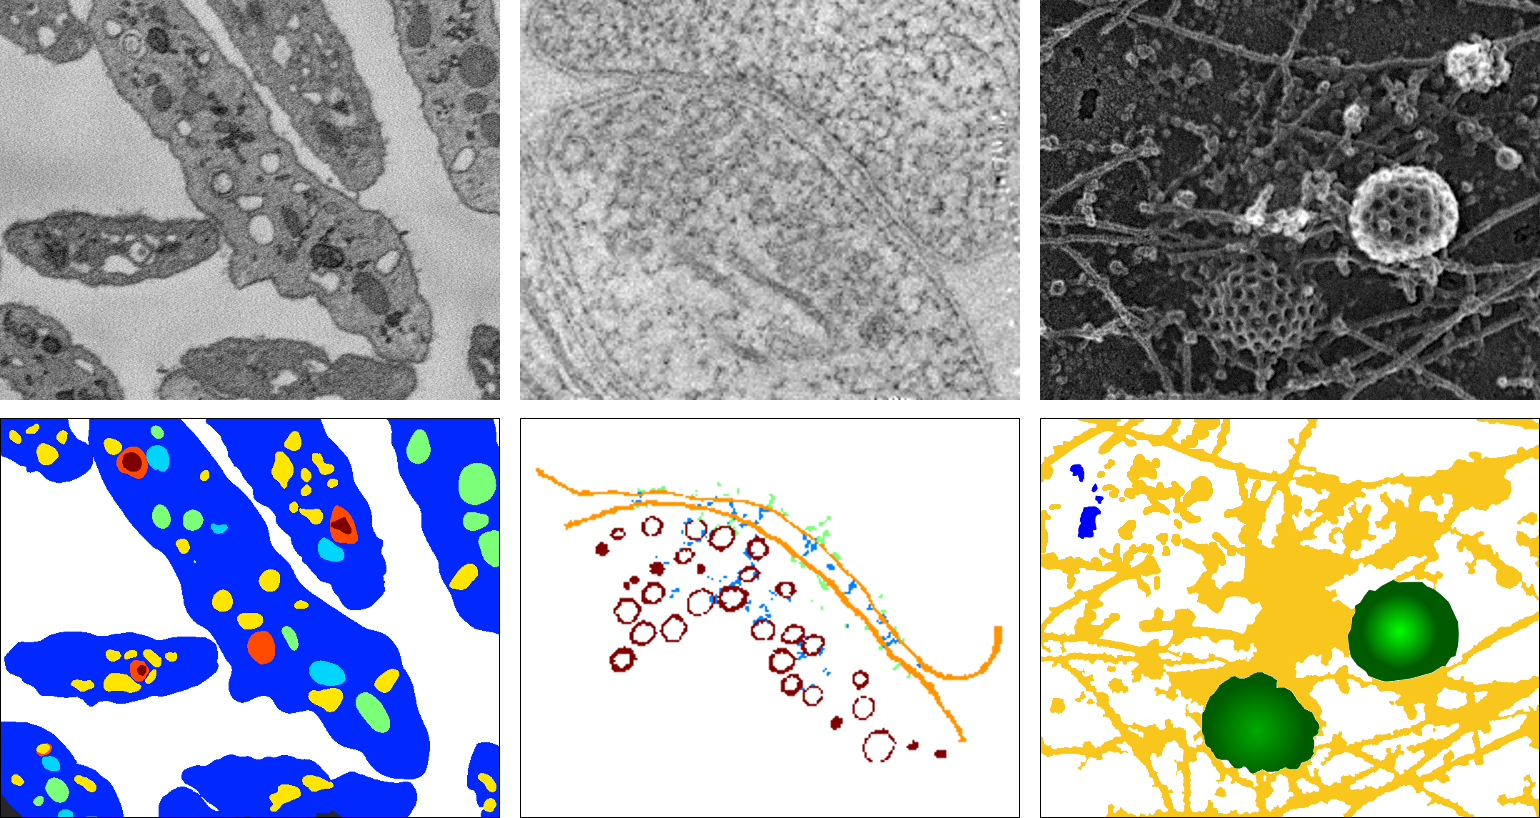
\includegraphics[width=\linewidth]{fig/segmentationintroshort.png}
\caption{Sample EM images, and their semantic segmentations. \textbf{Left}: SBF-SEM image of platelet cells. \textbf{Center}: TEM tomographic image of synaptic tissue, courtesy of NINDS Laboratory of Neurobiology. \textbf{Right}: Platinum-replica TEM tomographic image of a HeLa cell wall, courtesy of the NHLBI Taraska Lab.}
\end{figure}
\end{center}

\begin{tcolorbox}[title=Segmentation Challenges]
\begin{itemize}
\item Training \emph{label generation} is tedious, and experts may disagree.
\item Different EM hardware + sample combinations create \emph{many image types}.
\item Segmentation automation difficulty is highly \emph{problem-dependent}.
\item \textbf{Goal}: A \emph{reproducible workflow} for effective neural segmentation architecture discovery, training, and usage.
\item \textbf{Goal}: Use that workflow to design \emph{problem-specific segmentation algorithms}.
\end{itemize}
\end{tcolorbox}

\end{column} 
% End of first column


\begin{column}{\sepwid}\end{column} % Empty spacer column


% Second column
\begin{column}{\onecolwid}

\begin{tcolorbox}[title=Network Architecture Design]
\begin{itemize}
\item Segmentation networks use combinations of \emph{multi-scale convolutional} modules.
\item Common modules: pooled convolution blocks, dilated convolution blocks, encoder-decoders, spatial pyramid pooling units, more.
\item \emph{Architecture design}: Construction of a computation graph which contains the variables trained during learning.
\item Segmentation network architecture design is a combinatorial search with a \emph{large state space} and \emph{expensive evaluations}.
% \item Module design decisions are represented as numeric \emph{hyperparameters}. 
% \item Simplifies manual and \emph{algorithmic network design}.
% \item Easily generate networks using \emph{multi-level} random hyperparameter sampling.
\end{itemize}
\end{tcolorbox}

\begin{center}
\begin{figure}
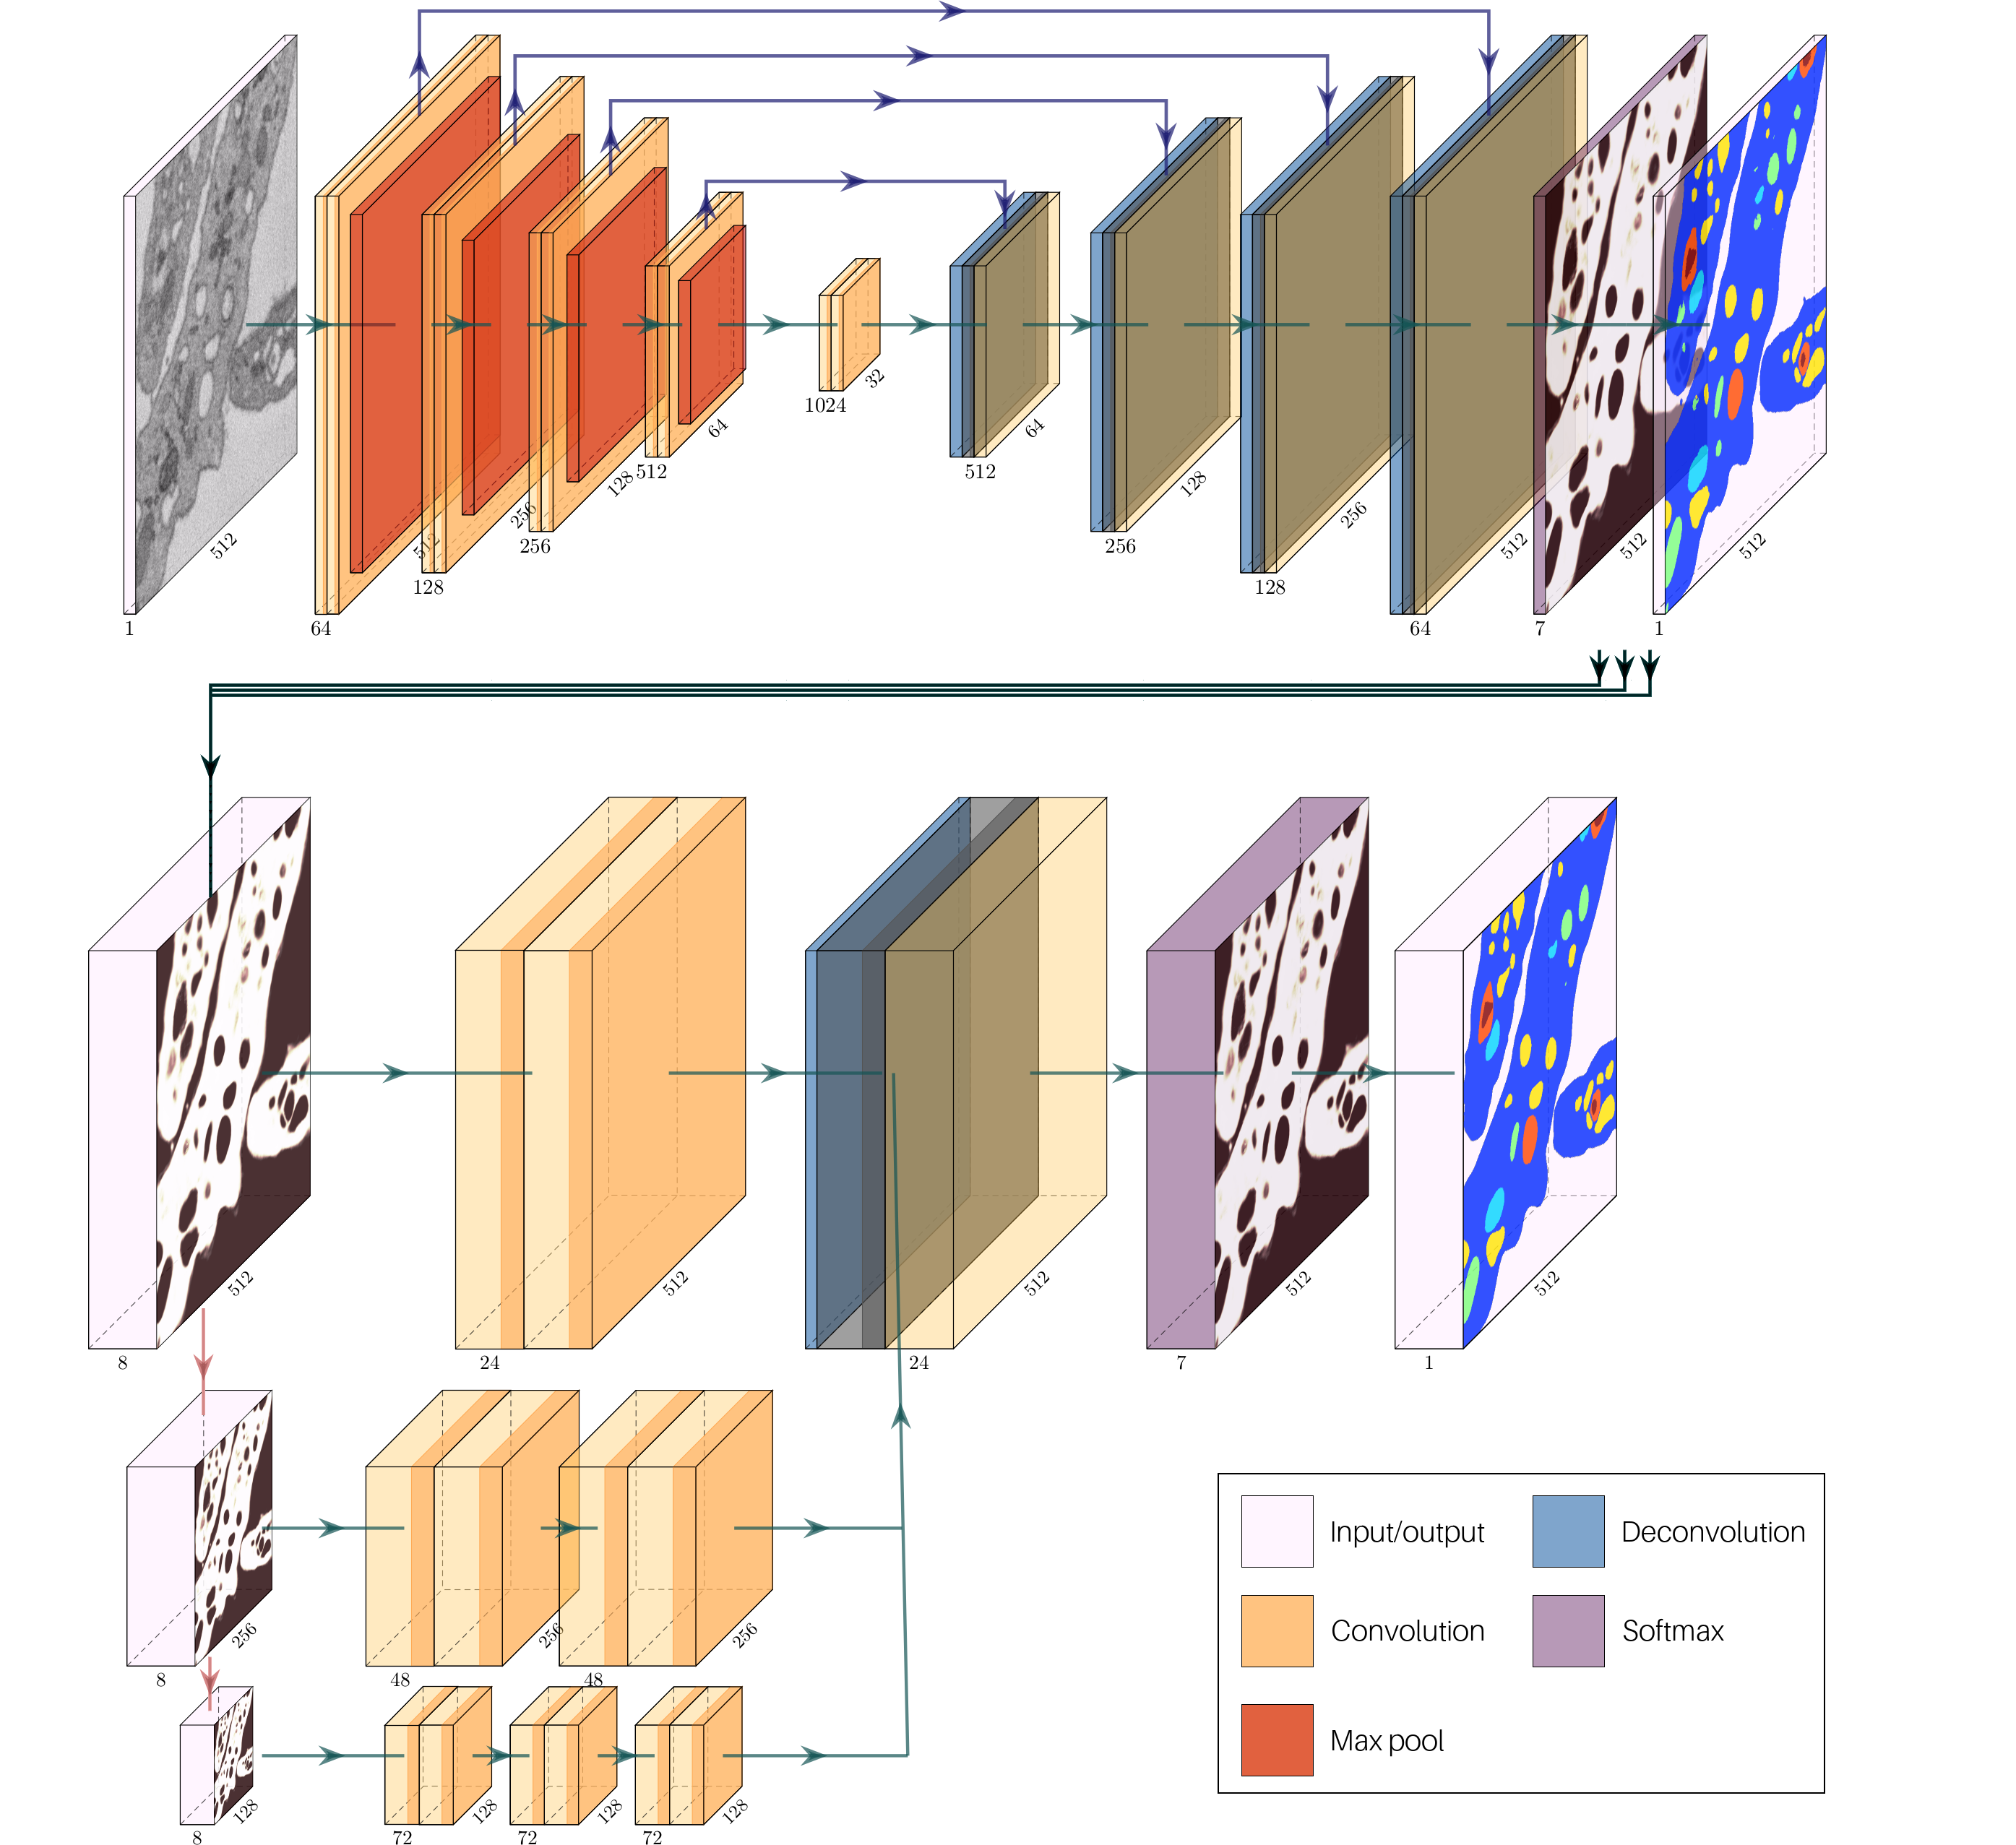
\includegraphics[width=\linewidth]{fig/fullnet-rearranged.png}
\caption{Example of a hybrid-3D + CRF-RNN segmentation network, of the type found most effective on 3D SBF-SEM data so far. More info in the next box.}
\end{figure}
\end{center}

\begin{tcolorbox}[title=Hybrid-3D Networks]
\begin{itemize}
\item \emph{2D vs 3D} tradeoffs: spatial context vs. memory usage, dealing with anisotropy along $z$ axis.
\item \emph{Hybrid-3D network}: Large 2D convolutional encoder-decoder module  forms intermediate predictions. Concatenated 2D predictions form input to a small 3D convolutional spatial pyramid module.
\item A 3D \emph{CRF-RNN} (conditional random field as recurrent neural network) module can be used as well.
\item Hybrid-3D + CRF-RNN architecture is currently the best performer.
% \item \emph{Goal}: Segment a platelet EM image into constituent cells and organelles (mitochondria, canalicular system, alpha granules, dense granules).
% \item Lab members manually segment a $50\times 800\times 800$ platelet volume for \emph{training data}.
% \item Train and evaluate 80 random encoder-decoder networks over 24 hours using \emph{Biowulf}, the NIH's HPC system. Compare with the original (Ronneberger et al., 2015) u-net.
% \item Form \emph{$N$-best} ensembles from the $N$ best networks, determine optimal $N$.
% \item Segment \emph{new data} using the best ensemble.
% \item Lab members \emph{correct} network output.
% \item Goal is \emph{workflow acceleration}, so compare correction time with manual segmentation time.
\end{itemize}
\end{tcolorbox}

\end{column}
% End of second column


\begin{column}{\sepwid}\end{column} % Empty spacer column


% Third column
\begin{column}{\onecolwid}

\begin{tcolorbox}[title=Architecture Design Algorithms]
\begin{itemize}
\item \emph{Algorithmic} architecture design: automatically search the architecture design space.
\item Observation: Segmentation networks form hierarchical \emph{module trees}: A tree of modules built up from repeated, simpler modules.
\item \emph{Random sampling} of module hierarchy trees finds effective segmentation architectures with modest computational resources.
\item Combine with other \emph{black box optimization} tools to improve parameters that do not alter the module hierarchy.
\item Run architecture search on NIH's \emph{Biowulf} using new distributed evaluation tools.
\item Diverse high-performing architectures are combined into \emph{ensembles} for improved prediction.
\end{itemize}
\end{tcolorbox}
\vspace{.1in}
\begin{center}
\begin{figure}
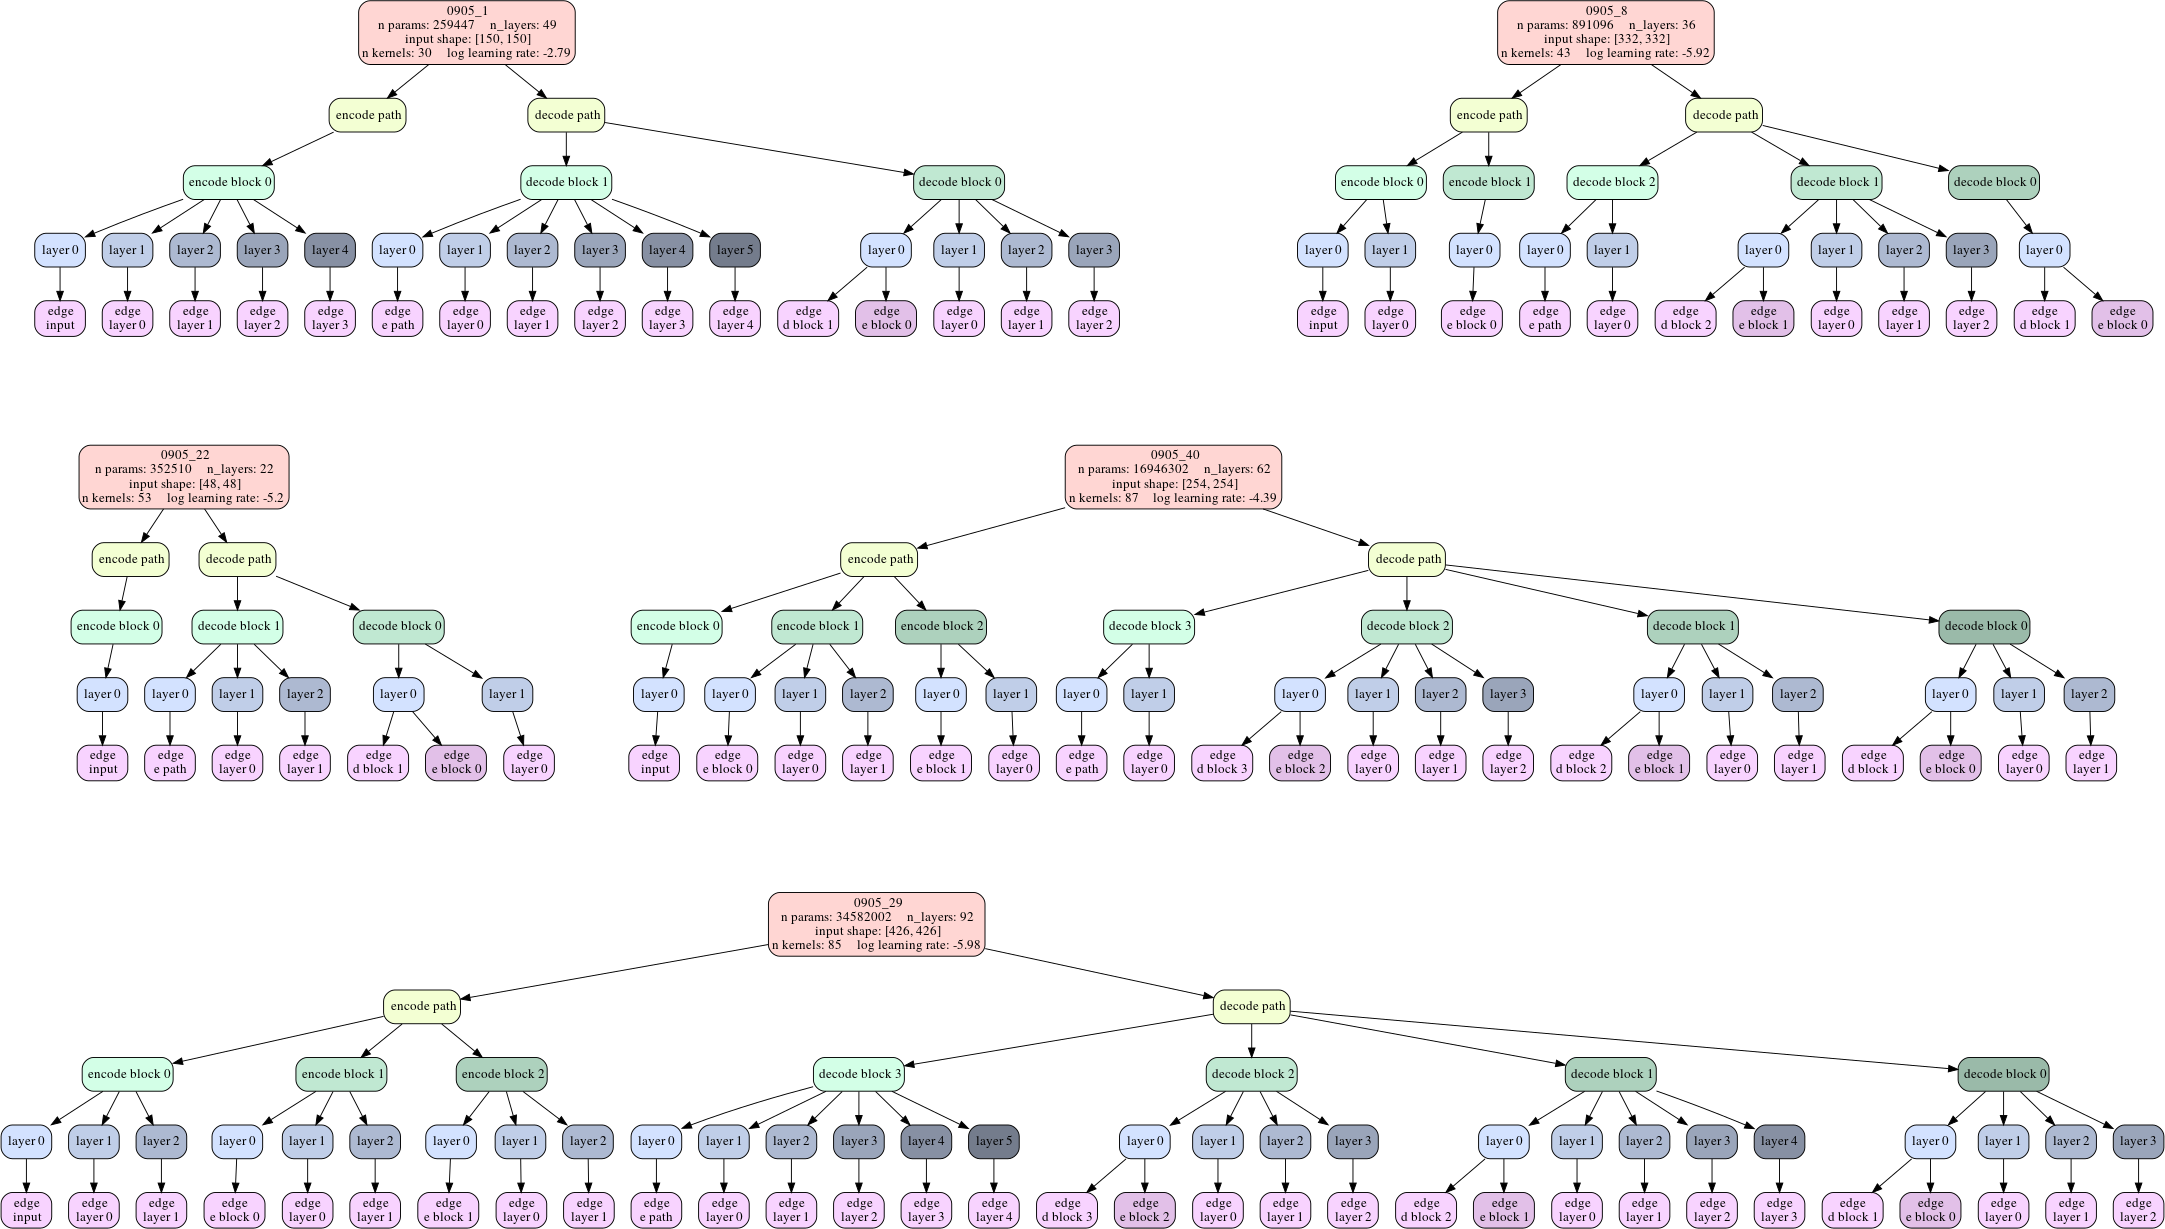
\includegraphics[width=\linewidth]{fig/ensemble.png}
\end{figure}

\vspace{.1in}

\begin{figure}
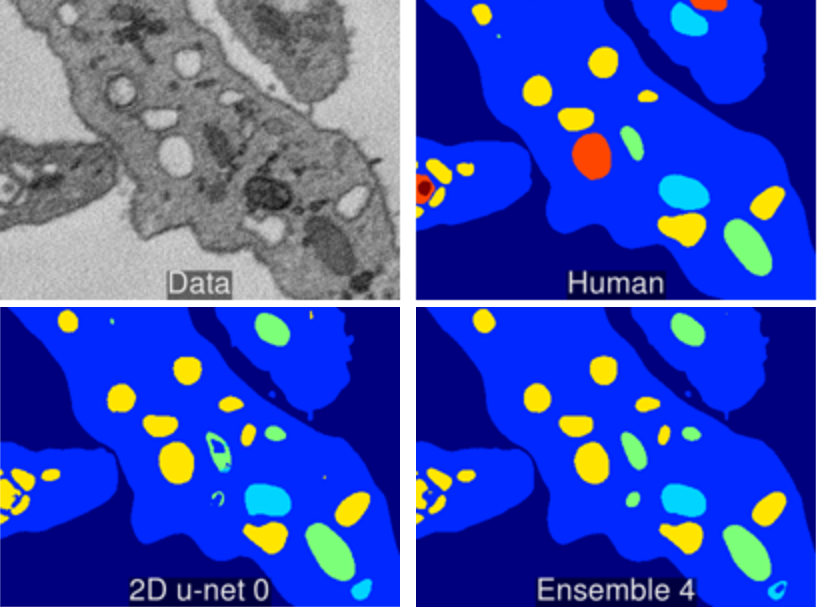
\includegraphics[width=\linewidth]{fig/top4.png}
\caption{(\textbf{Top}) A collection of randomly-generated module trees for 2D encoder-decoder networks. Each module forms part of a final computation graph. (\textbf{Bottom}) Importance of ensembling for segmentation algorithms. Data and human ground-truth labelings are compared with the single best network and the best network ensemble from 100 random 2D encoder-decoder networks.}
\end{figure}

\end{center}

\end{column}
% End of third column


\begin{column}{\sepwid}\end{column} % Empty spacer column


% Fourth column
\begin{column}{\onecolwid}

\begin{tcolorbox}[title=Conclusion]
\begin{itemize}
\item We built \textbf{high-performing 3D EM segmentation} algorithms with a new architecture which combines 2D and 3D convolutional processing modules.
\item Module architecture design made use of \emph{random module tree} sampling followed by \emph{black box} optimization.
\item Random sampling strategy produces high-performance segmentation networks and requires little machine learning expertise.
\item New scripting tools enable efficient, fault-tolerant distributed architecture search on Biowulf.
\item Resulting segmentation algorithms \emph{accelerate segmentation} for lab research workflows.
\item Challenges:
\begin{itemize}
\item \emph{End-to-end} training of large networks with model-parallel multi-GPU.
\item Deal with \emph{anomalies} in datasets not found in training data.
\end{itemize}
\end{itemize}
\end{tcolorbox}

\begin{tcolorbox}[title=Future Work]
\begin{itemize}
\item \emph{Robust segmentation}: Train a single segmentation model that works across multiple datasets. Requires transfer learning but also more.
\item \emph{New public dataset}: Currently assembling a collection of annotated EM image volumes for release to the machine learning community.
\item Use a \emph{correction-training feedback loop} to produce large amounts of labeled training data.
\item Combine \emph{instance and semantic} segmentation algorithms to increase usefulness of segmentation tools for researchers.
\item Work with collaborators to \emph{improve segmentation software} from preprocessing through data visualization.
\end{itemize}

\end{tcolorbox}

\begin{tcolorbox}[title=Acknowledgements]
\begin{itemize}
\item This work was supported by the intramural research program of the National Institute of Biomedical Imaging and Bioengineering.

\item This work made use of the computational resources of the NIH HPC Biowulf cluster. (https://hpc.nih.gov)

\item \textbf{View this poster online} at (\emph{https://leapmanlab.github.io/umd2019.pdf}).
\end{itemize}
\end{tcolorbox}

\end{column}
% End of fourth column

\end{columns}

\end{frame}

\end{document}

